\section{Experiments and Evaluation}
\label{sec4}

\subsection{Experimental Setup}

\noindent This subsection outlines the experimental environment and software configurations adopted to ensure methodological rigor and reproducibility of the results. 
All experiments were conducted within a virtualized environment deployed on a single physical host. 
The virtualization platform used was VirtualBox version 5.2.42, running a 64-bit Ubuntu 24.10 virtual machine instance. 
The virtual machine was allocated 4 GB of memory and operated on an Intel i5-13500H CPU. 
The Python environment version 3.12.3 was employed to support tasks including network emulation, data processing, control plane implementation, and machine learning model training and inference.

For network emulation, Mininet 2.3.1~\cite{Mininet} was utilized to construct the network topology and manage traffic scheduling. 
The data plane was implemented using the BMv2 software switch. 
P4 programs were developed following the P4\textsubscript{16} language specification and compiled with the p4c compiler version 1.2.4.15, targeting the official V1Model 20200408 architecture. 
The control plane was realized using P4Runtime version 1.3.0, facilitating flow table configuration, register access, and message handling. 
Traffic generation was handled by iPerf 2.1.9~\cite{iPerf}, which produced consistent TCP/UDP traffic. 
In addition, Scapy version 2.5.0~\cite{SCAPY} was employed to parse PCAP files and replay traffic, allowing fine-grained control over packet rates and inter-packet intervals during data collection.

\rev{
It is worth noting that alternative software switches such as OVS are not used for experimental comparison in this study. 
Although OVS is widely deployed in virtualized environments, it does not natively support the P4 programming model, nor does it provide mechanisms equivalent to P4 registers, digest messages, or in-switch stateful processing required for event-driven monitoring and proactive reporting. 
Similarly, performance-optimized variants such as OVS with DPDK (Data Plane Development Kit)~\cite{DPDK} primarily focus on accelerating packet I/O throughput, but still lack native support for P4-based programmable pipelines and control plane driven asynchronous telemetry primitives. 
As a result, a direct comparison between BMv2 and OVS or OVS with DPDK would be methodologically inappropriate for evaluating the functional correctness and adaptive behavior of P4-based monitoring mechanisms.
}

The experimental topology is illustrated in Figure~\ref{topo}, consisting of two BMv2 software switches and two host nodes, with each switch connected to one host. 
The switches were directly interconnected and linked to a centralized controller. 
A total of 100 flows were configured during the experiments, leading to a P4 register index width of 7 bits ($\lceil \log_2 100 \rceil$).

\begin{table*}[!t]
    \centering
    \caption{Summary of experimental environment and software configurations.}
    \label{env_table}
    \begin{tabular}{p{0.32\textwidth} p{0.48\textwidth}<{\raggedright}}
        \toprule
        \textbf{Category} & \textbf{Configuration Details} \\
        \midrule
        \textbf{Host Hardware} & Intel i5-13500H CPU, 4 GB RAM \\
        \textbf{Virtualization} & VirtualBox 5.2.42, Ubuntu 24.10 (64-bit VM) \\
        \textbf{Python Environment} & Python 3.12.3 \\
        \textbf{Network Emulation} & Mininet 2.3.1, BMv2 switch \\
        \textbf{P4 Compilation} & P4\textsubscript{16}, V1Model 20200408, p4c 1.2.4.15 \\
        \textbf{Control Plane} & P4Runtime 1.3.0 \\
        \textbf{Traffic Generation} & iPerf 2.1.9, Scapy 2.5.0 \\
        \textbf{ML Frameworks} & scikit-learn 1.5.2 (SVM), LightGBM 4.6.0, XGBoost 1.7.6 \\
        \textbf{Hyperparameter Tuning} & Optuna 4.2.1 \\
        \textbf{Configured Flow Count} & 100 flows; register index width = 7 bits \\
        \bottomrule
    \end{tabular}
\end{table*}

To facilitate quick reference to the experimental setup, Table~\ref{env_table} summarizes the hardware specifications, virtualization settings, network emulation tools, and machine learning frameworks used throughout the evaluation. 
The selection and configuration of these components were designed to ensure that the results are both reproducible and representative of realistic deployment conditions.

\begin{figure}[!t]
    \centering
    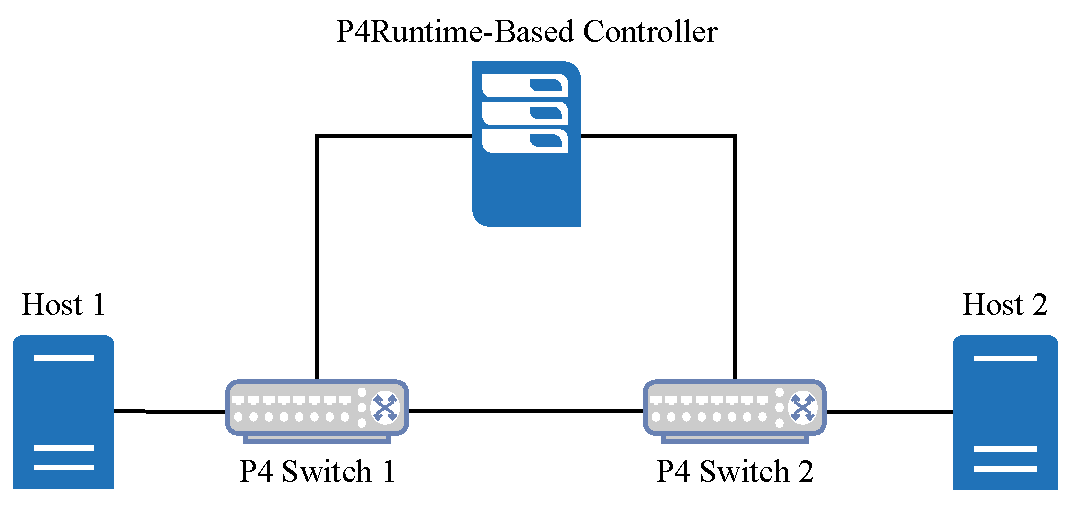
\includegraphics[width=0.48\textwidth]{./figures/topo.pdf}
    \caption{Network topology.}
    \label{topo}
\end{figure}

The training and hyperparameter optimization of machine learning models relied on the following software packages: scikit-learn 1.5.2~\cite{Scikit-learn} was used to construct and evaluate the SVM models; LightGBM 4.6.0 and XGBoost 1.7.6 were employed to implement lightweight and high-efficiency gradient boosting frameworks, respectively. 
Hyperparameter tuning was conducted using Optuna version 4.2.1~\cite{Optuna}, enabling automated search strategies to enhance model performance.

\rev{
To further support transparency and reproducibility, the complete source code, experimental scripts, and configuration files used in this study are publicly available in an open-access repository~\cite{MAT4PM}. 
The repository includes the P4 data plane programs, controller-side implementation code, machine learning training and inference code, as well as Mininet topology scripts and traffic generation configurations. 
All experiments reported in this paper can be reproduced under the specified software environment detailed in this subsection.
}

\subsection{Model Training Details}
\label{subsection42}

\noindent
% To comprehensively evaluate the adaptive threshold inference capabilities of the MAT4PM system across different learners, three mainstream regression models---XGBoost, LightGBM, and SVM---are trained using the labeled dataset collected in the experiments. 
\rev{Three mainstream regression models, namely XGBoost, LightGBM, and SVM, are trained on the labeled dataset to evaluate the adaptive threshold inference capability of MAT4PM.} 
XGBoost is a widely adopted ensemble learning algorithm based on gradient boosted decision trees, known for its high predictive accuracy and scalability. 
LightGBM is a histogram-based boosting framework designed for fast training and low memory usage, particularly suitable for real-time applications. 
% SVM is effective for capturing nonlinear relationships through kernel-based learning, offering strong generalization even with limited training data. 
\rev{SVM captures nonlinear relationships through kernel-based learning and maintains robust generalization with limited training data.} 
All models are developed using supervised learning, with the reported byte rate (\texttt{reported\_bps}) and packet rate (\texttt{reported\_pps}) as input features, and the optimal monitoring threshold (\texttt{optimal\_prdm}) as the regression target. 
The dataset is randomly split into training and validation sets at an 8:2 ratio. 
The training set is used for model fitting, while the validation set is utilized for hyperparameter tuning and performance evaluation.

To enhance model performance and reduce manual tuning bias, Bayesian optimization is applied for automated hyperparameter selection. 
Each model is trained over 100 trials (\texttt{n\_trials} = 100) within a predefined search space, with mean squared error (MSE) on the validation set serving as the evaluation metric. 
The final configurations obtained through Bayesian optimization are summarized in Table~\ref{tab:hyperparams}, which presents key hyperparameter settings for each model. 
This tabular presentation facilitates a clear comparison of tuning results across model types, supporting reproducibility and implementation transparency.

\begin{table}[!t]
    \centering
    \caption{Optimal hyperparameter configurations for each machine learning model.\label{tab:hyperparams}}
    \begin{tabular}{p{0.14\textwidth} p{0.18\textwidth} p{0.06\textwidth}<{\centering}}
        \toprule
        \textbf{Model} & \textbf{Hyperparameter} & \textbf{Value} \\
        \midrule
        \multirow{8}{*}{\textbf{XGBoost}} 
        & \texttt{n\_estimators} & 359 \\
        & \texttt{learning\_rate} & 0.0134 \\
        & \texttt{max\_depth} & 3 \\
        & \texttt{gamma} & 0.2812 \\
        & \texttt{subsample} & 0.6055 \\
        & \texttt{colsample\_bytree} & 0.7713 \\
        & \texttt{reg\_alpha} & 0.0077 \\
        & \texttt{reg\_lambda} & 0.3537 \\
        \midrule
        \multirow{7}{*}{\textbf{LightGBM}} 
        & \texttt{num\_leaves} & 31 \\
        & \texttt{learning\_rate} & 0.1301 \\
        & \texttt{feature\_fraction} & 0.7988 \\
        & \texttt{bagging\_fraction} & 0.8462 \\
        & \texttt{min\_data\_in\_leaf} & 36 \\
        & \texttt{reg\_alpha} & 0.3431 \\
        & \texttt{reg\_lambda} & 0.0394 \\
        \midrule
        \multirow{4}{*}{\textbf{SVM (Sigmoid)}} 
        & \texttt{C} & 152.5498 \\
        & \texttt{epsilon} & 0.8845 \\
        & \texttt{gamma} & 0.0192 \\
        & \texttt{degree} & 4 \\
        \bottomrule
    \end{tabular}
\end{table}

To assess the deployability of each model in real-world systems, memory consumption and prediction latency are measured. 
Upon loading, the memory footprint of each model is recorded as follows: XGBoost—30.99 KB, LightGBM—13.89 KB, and SVM—36.24 KB. 
These values indicate that all models exhibit minimal memory overhead, rendering them suitable for deployment on resource-constrained switches, controllers, or edge nodes.

Inference efficiency is further evaluated using the Python \texttt{timeit} module. 
Each model performs 1000 consecutive predictions after loading, and the execution time for each inference is recorded. 
The distribution of individual prediction times is illustrated in Figure~\ref{PredictionTimeCostsLine}. 
% The results show that the majority of predictions are completed within 1~ms, with only occasional outliers. 
\rev{Most predictions are completed within 1~ms, with only occasional outliers.} 
Specifically, XGBoost, LightGBM, and SVM achieve maximum prediction latencies of 4.545~ms, 3.920~ms, and 2.282~ms respectively, all significantly under the 5~ms soft real-time threshold empirically defined for this application scenario.

To better visualize the central tendency and variance in prediction latency, boxplots are generated for all models, as shown in Figure~\ref{PredictionTimeCostsBox}. 
Outliers are excluded based on default settings, and the mean inference time is marked by green triangles. 
The average prediction time is 0.949~ms for XGBoost, 0.771~ms for LightGBM, and 0.789~ms for SVM. 
These results confirm the suitability of all three models for real-time inference in MAT4PM, meeting the latency requirements of dynamic SDN monitoring scenarios.

\begin{figure}[!t]
    \centering
    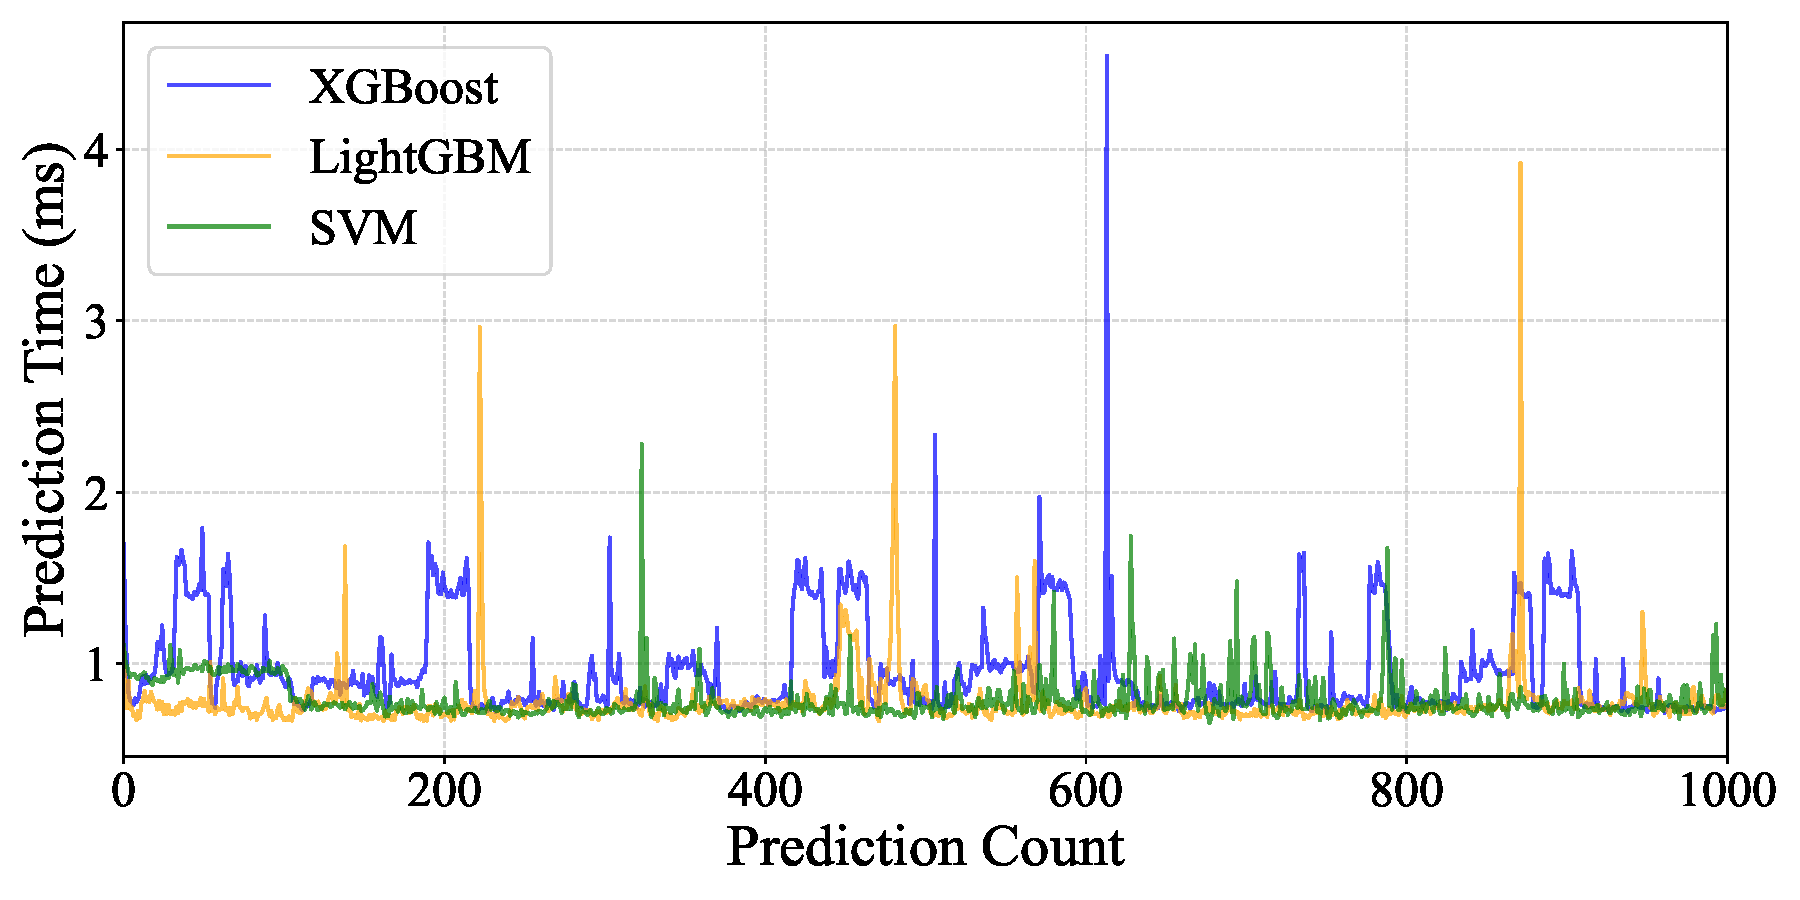
\includegraphics[width=0.48\textwidth]{./figures/PredictionTimeCostsLine.pdf}
    \caption{Line chart comparing the prediction time costs.}
    \label{PredictionTimeCostsLine}
\end{figure}

\begin{figure}[!t]
    \centering
    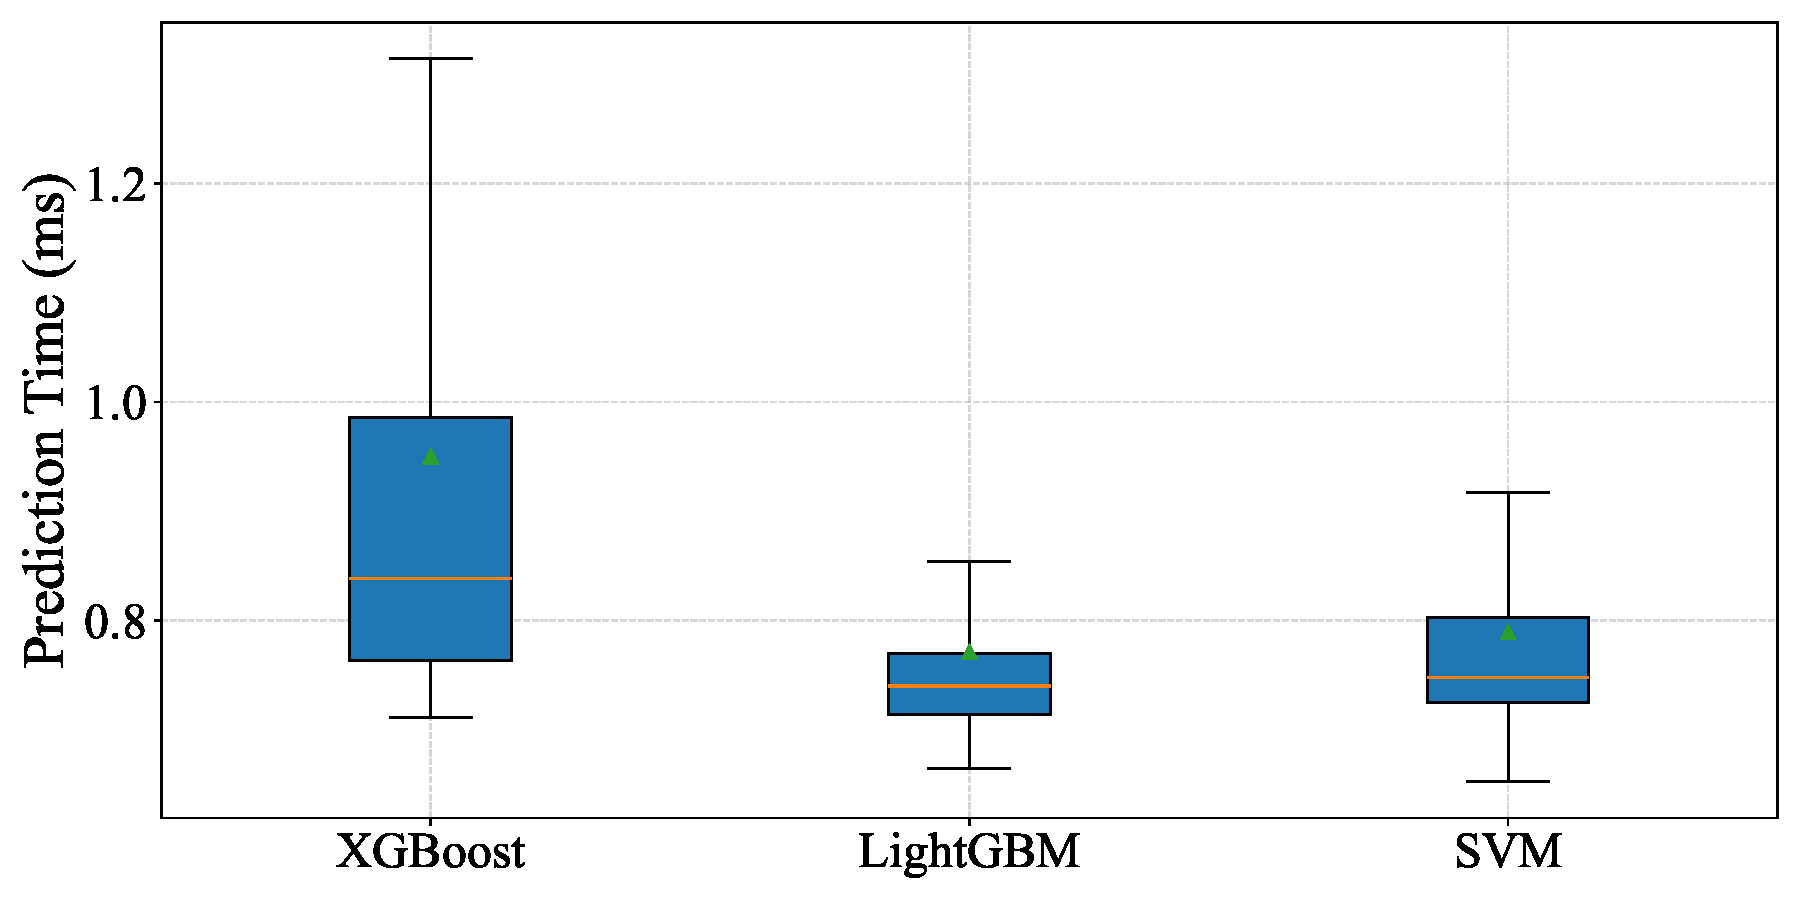
\includegraphics[width=0.48\textwidth]{./figures/PredictionTimeCostsBox.pdf}
    \caption{Boxplot comparing the prediction time costs.}
    \label{PredictionTimeCostsBox}
\end{figure}

\subsection{Evaluation Metrics}

\noindent To comprehensively assess the performance of various monitoring schemes---including fixed-threshold and machine learning-based adaptive thresholding methods---under identical traffic conditions, three core evaluation metrics are defined. 
These metrics respectively measure the reporting error rate, communication overhead, and overall system cost, enabling quantitative comparison across key dimensions.

The reporting error rate $\varepsilon$ evaluates the accuracy of reported traffic statistics and is formally defined as:
\begin{equation}
    \varepsilon = \frac{1}{N} \sum_{i=1}^{N} \left| \frac{r_{i}^{reported} - r_{i}^{true}}{r_{i}^{true}} \right|,
\end{equation}
where $N$ denotes the number of reporting events, and $r_{i}^{reported}$ and $r_{i}^{true}$ represent the reported and actual rates, respectively, at the $i$-th instance. 
This metric corresponds to the average of relative errors across all reporting events. 
A lower value of $\varepsilon$ indicates a higher fidelity of the monitoring system in capturing the true network dynamics and is thus a critical measure of monitoring accuracy.

The communication overhead $C$ quantifies the control plane burden introduced by monitoring, defined as the average number of reports per unit time. 
The total number of reporting events during the test period is divided by the total test duration to yield the raw reporting frequency. 
For consistency with the error metric and for multi-objective optimization, the overhead is normalized with respect to a predefined upper bound $C_{max}=50$ (i.e., a maximum of 50 reports per second):
\begin{equation}
    C_{norm} = \frac{C_{raw}}{C_{max}},
\end{equation}
where the raw overhead $C_{raw}$ is computed as:
\begin{equation}
    C_{raw} = \frac{R}{T},
\end{equation}
with $R$ denoting the total number of reporting events during the evaluation period, and $T$ representing the total duration. 
A lower $C_{norm}$ implies a reduced communication burden, which alleviates the processing pressure on the controller and reduces bandwidth consumption.

To balance monitoring accuracy against communication efficiency, a composite metric $\text{Cost}$ is introduced, defined as a weighted sum of the reporting error $\varepsilon$ and the normalized communication overhead $C_{norm}$:
\begin{equation}
    \text{Cost} = \alpha \cdot \varepsilon + \beta \cdot C_{norm},
\end{equation}
where $\alpha$ and $\beta$ are weighting coefficients corresponding to the relative importance of accuracy and overhead.
For consistency with dataset construction, the values $\alpha = 0.6$ and $\beta = 0.4$ are adopted, reflecting a greater emphasis on monitoring precision. 
Minimizing $\text{Cost}$ ensures that the system achieves a favorable trade-off between accuracy and efficiency, aligning with practical deployment objectives.

During the evaluation process, each monitoring scheme is independently tested over a 30-second period under identical traffic inputs. 
This uniform test condition eliminates external variability and ensures fair comparability across different methods. 
The proposed tri-metric framework allows for multi-faceted, systematic assessment of each scheme in terms of accuracy, efficiency, and overall cost-effectiveness, thereby providing a robust analytical foundation for subsequent performance analysis.

\subsection{Experimental Results and Analysis}

\noindent This section presents and analyzes the experimental results of MAT4PM across several key dimensions, including its impact on throughput performance and the effectiveness of the dynamic threshold control strategy powered by machine learning models. 
\rev{In addition to reporting mean values, statistical variability is explicitly characterized through confidence intervals (CIs) and error bars to provide a more comprehensive assessment of performance stability.}

Figure~\ref{loss_mbps} illustrates the variation in switch throughput after the integration of the MAT4PM monitoring mechanism. 
To evaluate the potential performance overhead introduced by the monitoring logic on the data plane, TCP throughput was measured using the iPerf tool in repeated trials. 
Each trial was conducted under two conditions: without the monitoring module (baseline) and with MAT4PM enabled while monitoring varying proportions of traffic. 
In the testbed, Host~2 operated as an iPerf server receiving a continuous 30-second TCP stream from Host~1, while the MAT4PM logic was deployed on the intermediate switch, Switch~2. 
By adjusting the percentage of monitored flows, the impact on overall throughput was observed. 
The blue dashed line in the figure represents the maximum throughput achieved without monitoring, while the orange solid line shows the measured throughput under different monitoring intensities. 
As the monitored traffic ratio increases, a gradual decline in throughput is observed. 
When 100\% of the traffic is monitored, throughput of MAT4PM decreases to 21.0 Mbps, approximately 13.2\% lower than the baseline of 24.2 Mbps. 
% This performance degradation is primarily attributed to the additional computational cost introduced by monitoring logic in the ingress pipeline, where each monitored packet triggers read and write operations across four registers (responsible for storing thresholds, byte counters, packet counters, and reporting timestamps). 
\rev{This performance degradation is primarily attributed to the additional computational cost introduced by the monitoring logic in the ingress pipeline. 
Each monitored packet triggers read and write operations across four registers, which store thresholds, byte counters, packet counters, and reporting timestamps.} 
As the monitoring coverage expands, the frequency of register access increases, which in turn negatively impacts the packet processing rate of the switch. 
Notably, this throughput impact aligns with state-of-the-art monitoring frameworks such as PPM \cite{10623873} and FlowStalker \cite{8761197}, which exhibit 13.05\% and 12\% throughput reduction under full traffic coverage.

\begin{figure}[!t]
    \centering
    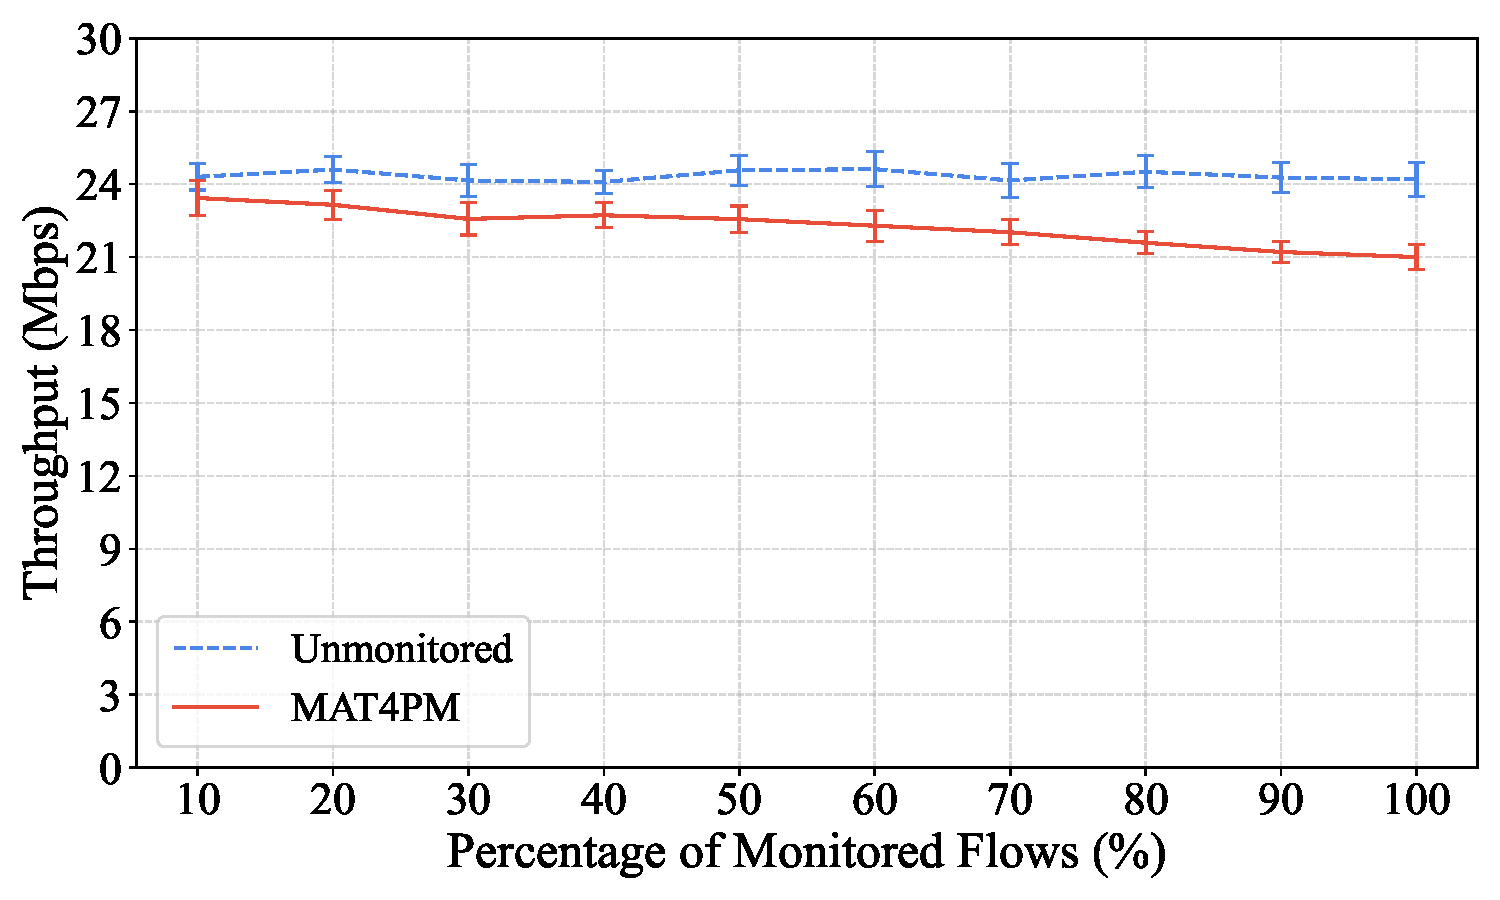
\includegraphics[width=0.49\textwidth]{./figures/loss_mbps.pdf}
    \caption{The impact of MAT4PM on throughput.}
    \label{loss_mbps}
\end{figure}

The subsequent experiments aim to evaluate the performance of machine learning-based dynamic threshold control strategies in real traffic scenarios, focusing on metrics including monitoring error, communication overhead, and overall cost. 
In this evaluation, Scapy was employed to generate a single flow with dynamic characteristics over a 30-second period, where the transmission rate changed every 5 seconds. 
Three dynamic threshold strategies based on machine learning models (XGBoost, LightGBM, and SVM) were compared against three fixed threshold baselines (with reporting intervals of 500~ms, 1000~ms, and 2000~ms).

Figure~\ref{monitoring} exemplifies the monitoring process under the XGBoost-based dynamic strategy. 
In this test, the traffic rates were set to 4 Mbps (0--5~s), 5.5 Mbps (5--10~s), 7.5 Mbps (10--15~s), 6 Mbps (15--20~s), 4 Mbps (20--25~s), and 7 Mbps (25--30~s). 
The blue solid line denotes the actual traffic rate, while the red dashed line indicates the corresponding reported rate. 
Overall, the two curves show close alignment across the entire test duration, indicating a high level of tracking accuracy. 
The system adaptively adjusts its reporting frequency based on traffic intensity. 
For instance, during the low-load period of 0--5 seconds, monitoring data were reported 12 times, whereas in the high-load interval of 10--15 seconds, the reporting frequency increased to 19. 
This behavior demonstrates a strong capacity for dynamic adaptation.

\begin{figure}[!t]
    \centering
    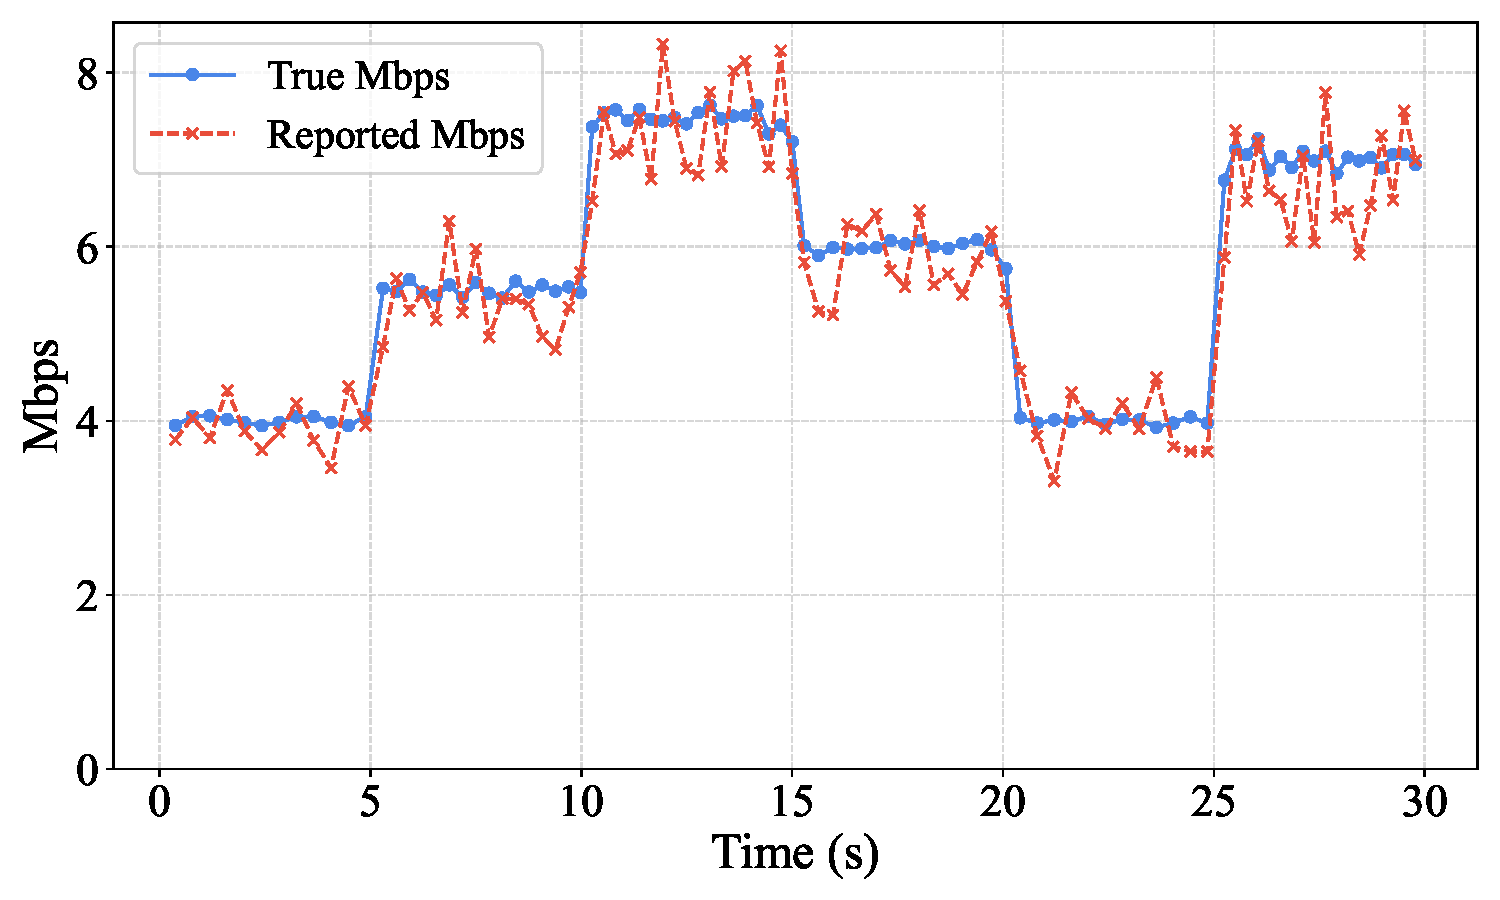
\includegraphics[width=0.49\textwidth]{./figures/monitoring.pdf}
    \caption{The monitoring process based on the XGBoost model.}
    \label{monitoring}
\end{figure}

To provide a consolidated view of monitoring performance, Table~\ref{summary_table} summarizes the key evaluation metrics---average monitoring error, reporting frequency, and total cost---for all six schemes. 
\rev{To characterize statistical variability, the reported monitoring error and total cost are expressed as mean values accompanied by their corresponding 95\% confidence intervals, computed over repeated measurements. 
This presentation provides insights into both average performance and result stability.}

\begin{table*}[!t]
    \centering
    \caption{Comparison of monitoring schemes in terms of error, reporting frequency, and total cost \rev{(mean $\pm$ 95\% CI)}.}
    \label{summary_table}
    \begin{tabular}{p{0.22\textwidth}<{\centering} p{0.18\textwidth}<{\centering} p{0.18\textwidth}<{\centering} p{0.16\textwidth}<{\centering}}
        \toprule
        \textbf{Scheme} & \textbf{Average Error (\%)} & \textbf{Reports per Second} & \textbf{Total Cost} \\
        \midrule
        \textbf{Fixed-500ms}
            & $ 9.1 \pm 0.31$
            & 1.967
            & $0.0703 \pm 0.0019$ \\
        \textbf{Fixed-1000ms}
            & $10.8 \pm 0.35$
            & 0.967
            & $0.0725 \pm 0.0021 $ \\
        \textbf{Fixed-2000ms}
            & $11.6 \pm 0.42$
            & \textbf{0.467}
            & $0.0733 \pm 0.0025$ \\
        \textbf{XGBoost}
            & $\mathbf{7.0 \pm 0.26}$
            & 3.033
            & $0.0663 \pm 0.0015$ \\
        \textbf{LightGBM}
            & $7.3 \pm 0.24$
            & 2.800
            & $\mathbf{0.0662 \pm 0.0015}$ \\
        \textbf{SVM}
            & $7.5 \pm 0.29$
            & 2.767
            & $0.0671 \pm 0.0018$ \\
        \bottomrule
    \end{tabular}
\end{table*}

These metrics are further examined and visualized in the subsequent figures. Figure~\ref{errors} presents the average monitoring error across the six schemes over the 30-second test duration. 
The fixed threshold configurations (500 ms, 1000 ms, and 2000 ms) yielded average errors of 9.1\%, 10.8\%, and 11.6\%, respectively. 
In contrast, the \mbox{XGBoost-}, \mbox{LightGBM-}, and SVM-based dynamic strategies achieved lower errors of 7.0\%, 7.3\%, and 7.5\%, respectively. 
\rev{In addition to mean error values, 95\% confidence intervals are depicted using error bars to reflect the variability of monitoring performance across repeated trials.} 
These results confirm the superiority of dynamic threshold control in improving monitoring accuracy compared to static schemes, \rev{and dynamic schemes exhibit relatively narrow confidence intervals, which indicates the stability and reliability of dynamic threshold control.}

\begin{figure}[!t]
    \centering
    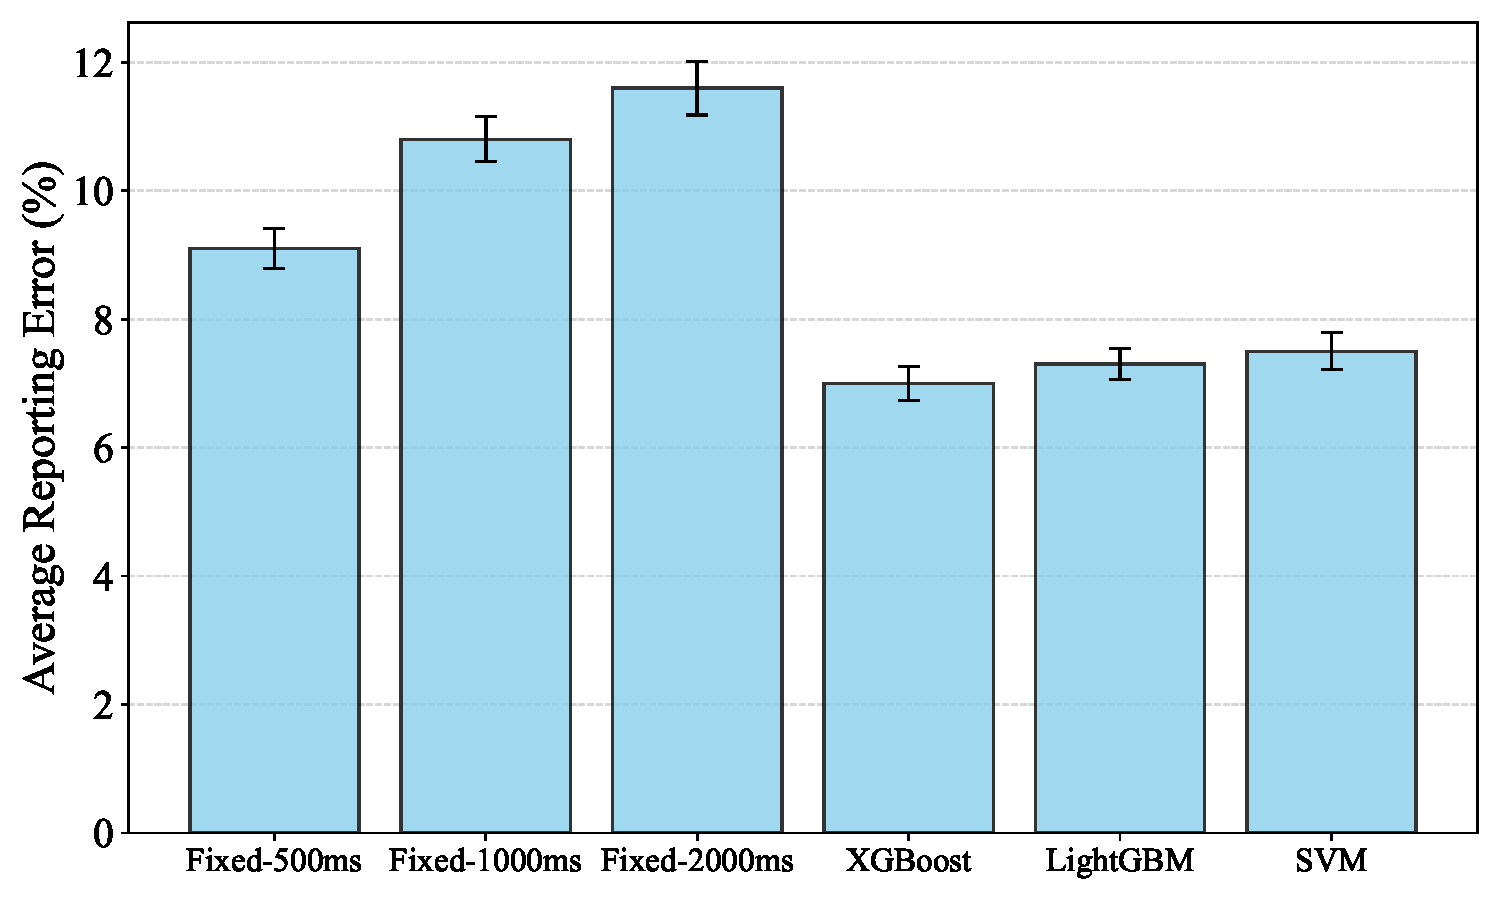
\includegraphics[width=0.49\textwidth]{./figures/errors.pdf}
    \caption{Average monitoring error of different schemes. \rev{Error bars indicate the 95\% CI.}}
    \label{errors}
\end{figure}

Figure~\ref{rps} provides the average number of reports per second for each scheme during the test period. 
The fixed interval strategies resulted in reporting rates of 1.967, 0.967, and 0.467 reports per second for the 500~ms, 1000~ms, and 2000~ms thresholds, respectively. 
It is important to note that a 500~ms reporting threshold does not guarantee an exact report every 500~ms. 
Instead, each report must be triggered by the arrival of at least one data packet; thus, the actual interval between consecutive reports is typically greater than or equal to the configured threshold. 
For instance, with a 500~ms threshold over a 30-second test duration, the total number of triggered reports was 59 rather than 60, yielding an observed average of 1.967 reports per second. 
The machine learning-based dynamic schemes achieved higher average reporting rates, with XGBoost, LightGBM, and SVM reporting monitoring data at 3.033, 2.800, and 2.767 times per second, respectively. 
Although these strategies incur increased communication frequency, they enable finer-grained monitoring under high traffic loads, thereby contributing to improved accuracy.

\begin{figure}[!t]
    \centering
    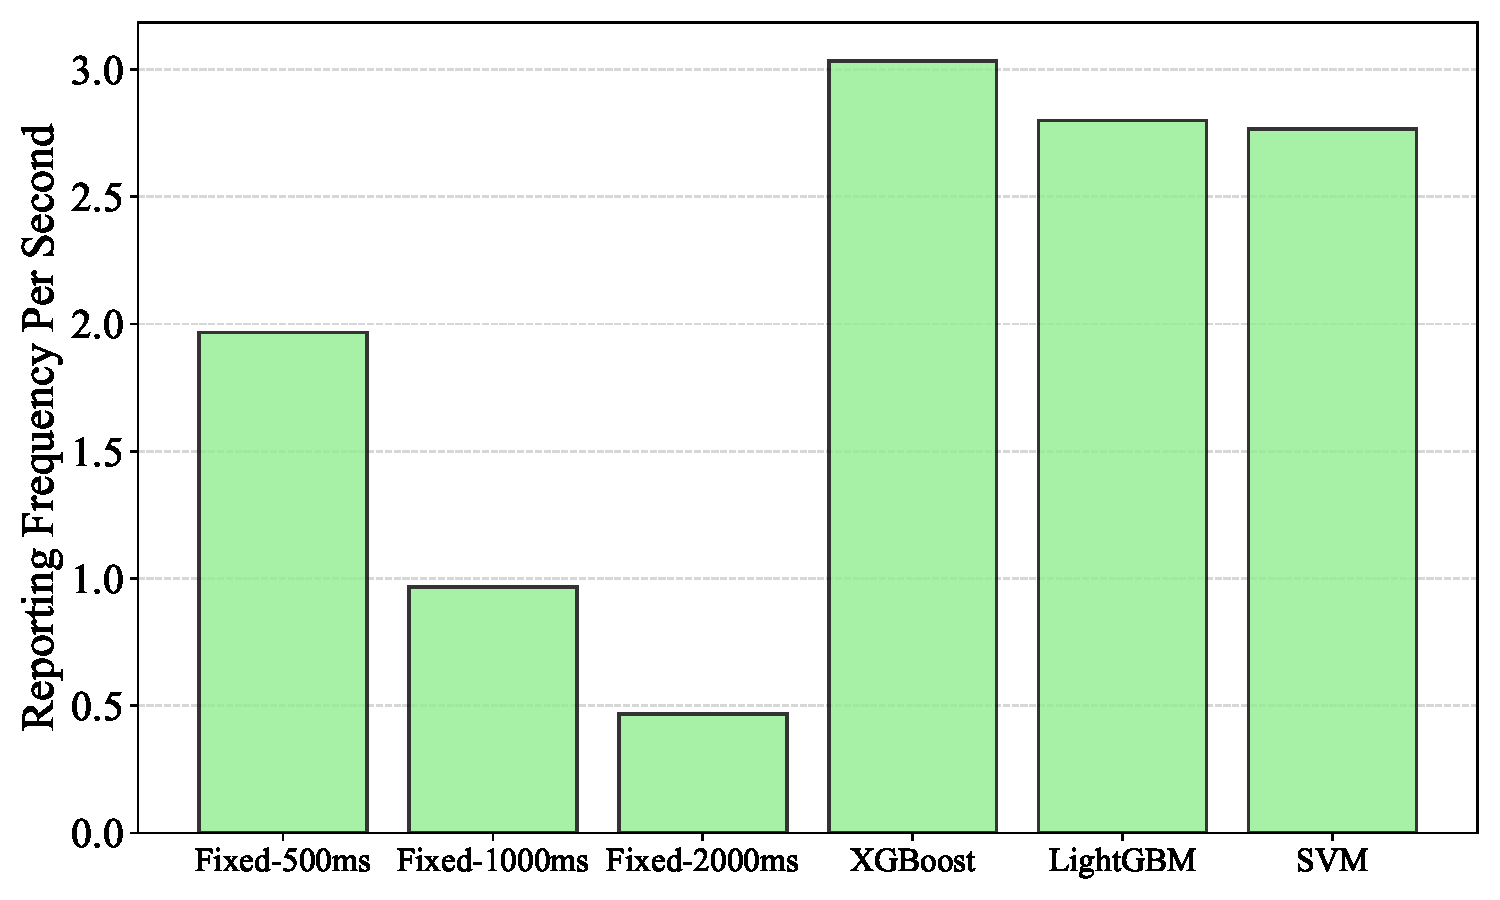
\includegraphics[width=0.49\textwidth]{./figures/rps.pdf}
    \caption{Average reporting frequency per second of different schemes.}
    \label{rps}
\end{figure}

To assess the trade-off between monitoring accuracy and communication cost, Figure~\ref{costs} reports the total cost for each scheme using weighted coefficients $\alpha=0.6$ and $\beta=0.4$. 
The fixed threshold strategies yielded total costs of 0.0703, 0.0725, and 0.0733 for the 500 ms, 1000 ms, and 2000 ms configurations, respectively. In comparison, the \mbox{XGBoost-,} \mbox{LightGBM-,} and SVM-based dynamic approaches achieved lower total costs of 0.0663, 0.0662, and 0.0671, respectively. 
These results reinforce the advantage of incorporating machine learning in striking a more favorable balance between accuracy and communication overhead, thereby reducing overall monitoring cost.

\begin{figure}[!t]
    \centering
    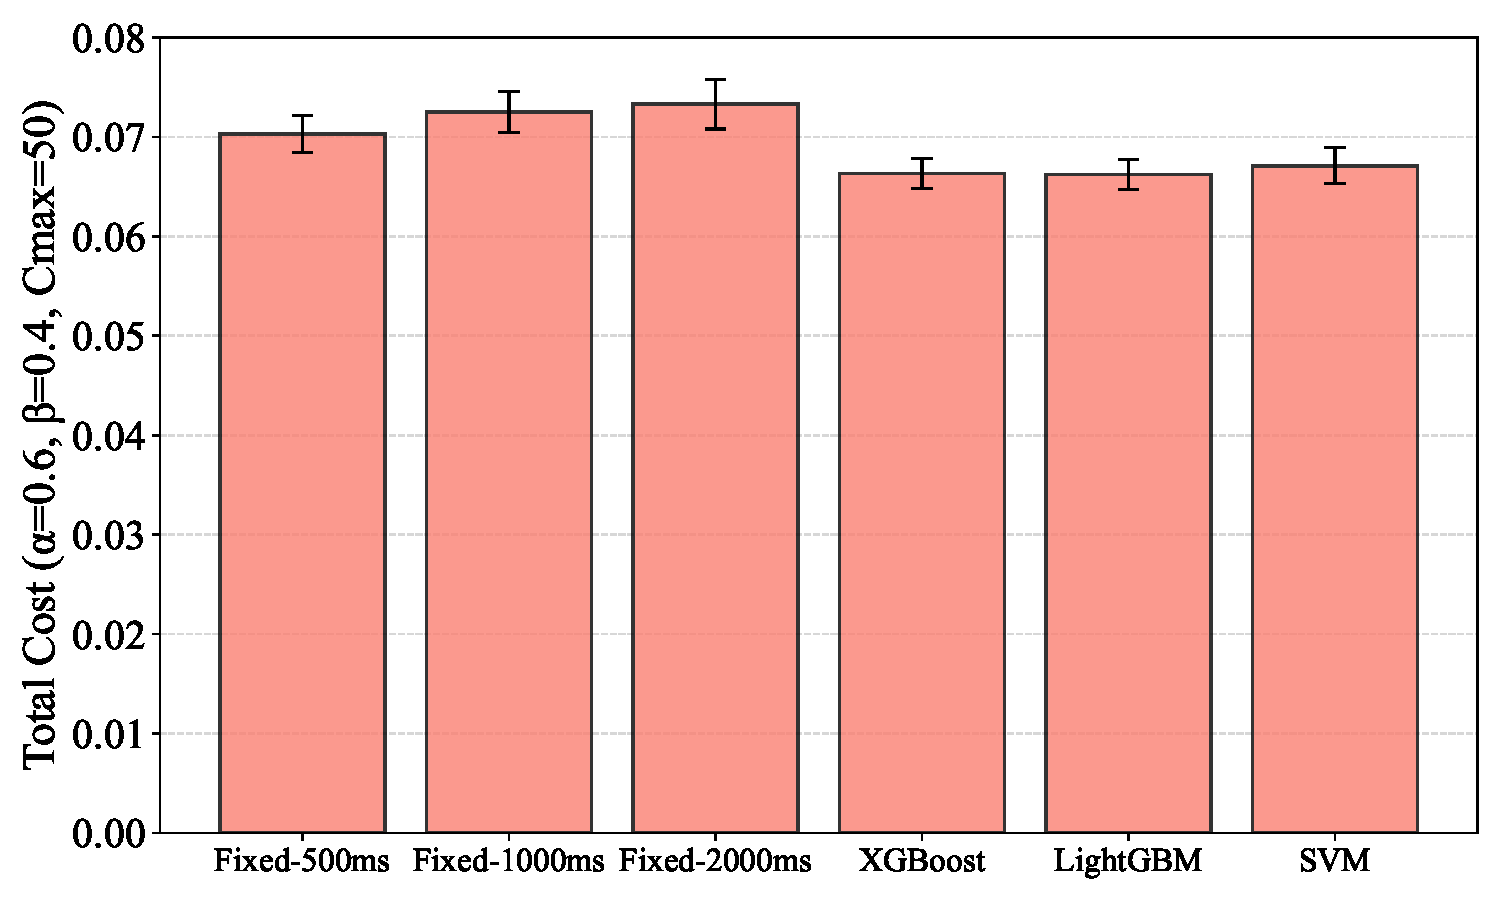
\includegraphics[width=0.49\textwidth]{./figures/costs.pdf}
    \caption{Total cost comparison among different monitoring schemes. \rev{Error bars indicate the 95\% CI.}}
    \label{costs}
\end{figure}

\rev{
Although Table~\ref{summary_table} reports quantitative differences among the three machine learning-based strategies, the primary objective of this evaluation is not to identify a universally optimal learning algorithm, but rather to demonstrate the effectiveness and robustness of machine learning-driven adaptive threshold control as a general paradigm.
}

\rev{
The three models considered in this study, namely XGBoost, LightGBM, and SVM, are selected as representative and widely adopted regression techniques with distinct learning characteristics. 
Tree-based ensemble models such as XGBoost and LightGBM are known for their strong capability in capturing nonlinear feature interactions and piecewise decision boundaries, which is particularly suitable for modeling the nonlinear relationship between traffic intensity and optimal monitoring thresholds~\cite{XGBoost,LightGBM}. 
This property partially explains why the XGBoost-based strategy achieves the lowest average monitoring error, while LightGBM attains the minimum total cost by maintaining a slightly lower reporting frequency under similar accuracy levels.
}

\rev{
In contrast, the SVM-based strategy exhibits marginally higher error and cost compared to the tree-based models. 
This behavior can be attributed to the sensitivity of kernel-based methods to hyperparameter selection and their limited flexibility in approximating abrupt changes when traffic patterns vary rapidly over short time scales~\cite{SVMs}. 
Nevertheless, the performance gap among the three models remains relatively small, and all machine learning-based approaches consistently outperform the fixed-threshold baselines on both average error and total cost.
}

\rev{
These observations suggest that the overall performance gains primarily stem from the introduction of adaptive, data-driven threshold adjustment, rather than reliance on a specific learning algorithm. 
Consequently, the proposed framework is compatible with a wide range of regression models, allowing practitioners to select learning techniques based on deployment constraints, interpretability requirements, or computational considerations.
}

\subsection{\rev{Scalability Analysis}}

\noindent \rev{
The proposed framework introduces machine learning driven adaptive threshold computation at the control plane, which inevitably incurs additional computational overhead compared to purely rule based monitoring schemes. 
To evaluate the scalability of the system under increasing monitoring scale, controller CPU utilization is examined along two dimensions: the number of concurrent flows and the number of monitored switches.
}

\subsubsection{\rev{Impact of Number of Flows}}

\rev{
The first experiment investigates the effect of flow scale on controller CPU usage. 
The experiment is conducted on the linear two switch topology illustrated in Figure~\ref{topo}, where telemetry data are collected from a single monitored switch. 
The number of active flows is gradually increased from 10 to 500, while all other parameters remain unchanged.
}

\rev{
Table~\ref{tab:cpu_flow} summarizes the statistical characteristics of controller CPU utilization under different flow counts, including the average, median, peak, minimum, and standard deviation. 
As shown in the table, CPU utilization increases steadily with the number of flows, rising from an average of 7.53\% at 10 flows to 64.0\% at 100 flows. 
Beyond 200 flows, the average CPU usage approaches a plateau around 72\%, and no further linear growth is observed even when the number of flows increases to 500.
}

\begin{table*}[!t]
    \centering
    \caption{\rev{Controller CPU utilization under different numbers of monitored flows.}}
    \label{tab:cpu_flow}
    \begin{tabular}{p{0.16\textwidth}<{\centering}
                    p{0.09\textwidth}<{\centering}
                    p{0.09\textwidth}<{\centering}
                    p{0.09\textwidth}<{\centering}
                    p{0.09\textwidth}<{\centering}
                    p{0.09\textwidth}<{\centering}}
        \toprule
        \textbf{\rev{Number of Flows}} & \textbf{\rev{Mean (\%)}} & \textbf{\rev{Median (\%)}} & \textbf{\rev{Peak (\%)}} & \textbf{\rev{Min (\%)}} & \textbf{\rev{Std. Dev.}} \\
        \midrule
        \rev{10 } & \rev{7.53 } & \rev{7.58 } & \rev{10.74} & \rev{3.79 } & \rev{1.74} \\
        \rev{20 } & \rev{14.28} & \rev{13.90} & \rev{18.32} & \rev{9.48 } & \rev{2.2 } \\
        \rev{50 } & \rev{34.05} & \rev{34.58} & \rev{42.33} & \rev{26.90} & \rev{3.57} \\
        \rev{100} & \rev{64.0 } & \rev{64.44} & \rev{76.45} & \rev{44.23} & \rev{7.38} \\
        \rev{200} & \rev{71.65} & \rev{71.71} & \rev{79.61} & \rev{61.28} & \rev{5.25} \\
        \rev{500} & \rev{73.07} & \rev{73.82} & \rev{80.24} & \rev{58.76} & \rev{4.53} \\
        \bottomrule
    \end{tabular}
\end{table*}

\rev{
To further illustrate the distribution and variability of CPU usage, Figure~\ref{cpu_usage_flow} presents boxplots of controller CPU utilization under different flow counts. 
The results indicate that both the median and interquartile range increase rapidly up to 100 flows, followed by a clear saturation trend. 
This behavior suggests that the controller reaches a stable operating regime in which available CPU resources become the dominant limiting factor.
}

\begin{figure}[!t]
    \centering
    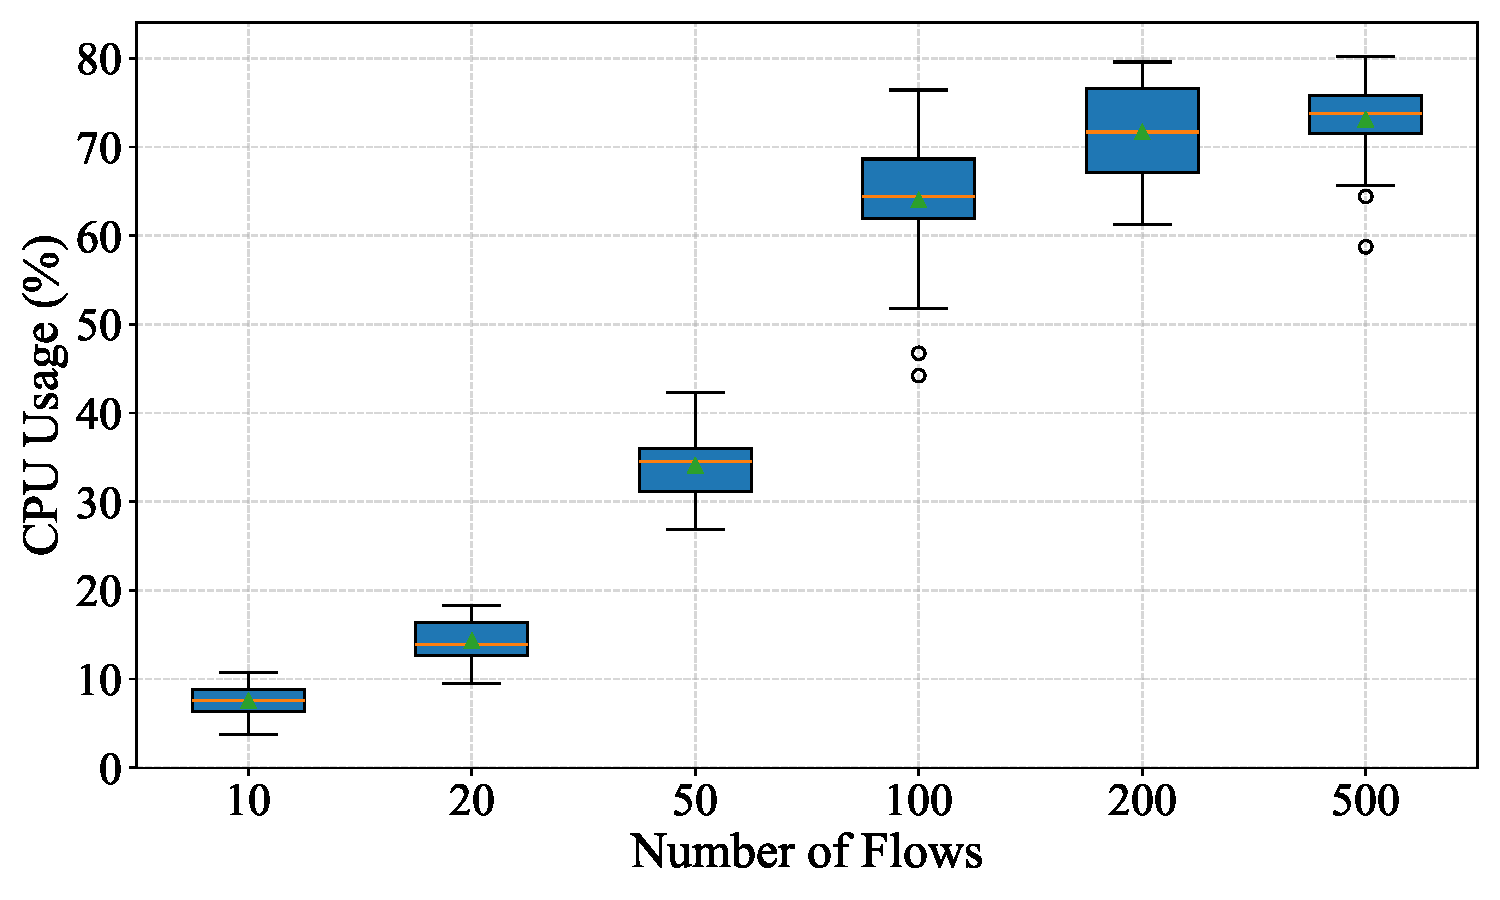
\includegraphics[width=0.49\textwidth]{./figures/cpu_usage_flow.pdf}
    \caption{\rev{Distribution of controller CPU usage under varying numbers of monitored flows.}}
    \label{cpu_usage_flow}
\end{figure}

\subsubsection{\rev{Impact of Number of Switches}}

\rev{
The second experiment evaluates scalability with respect to network size by increasing the number of monitored switches. 
The experiment linearly scales the topology from one to five monitored switches. 
Figure~\ref{topo} illustrates the baseline two-switch case. 
The number of active flows is fixed at 40, and the controller concurrently processes telemetry feedback from all monitored switches.
%Starting from the baseline topology shown in Figure~\ref{topo}, additional switches are incrementally added to form linear topologies with one to five monitored switches. 
%Throughout this experiment, the number of active flows is fixed at 40, and the controller concurrently processes telemetry feedback from all monitored switches.
}

\rev{
Table~\ref{tab:cpu_switch} reports the controller CPU utilization statistics under different numbers of switches. 
The results show that average CPU usage increases sharply when the number of switches grows from one to three, rising from 14.75\% to 65.76\%. 
When four or five switches are monitored concurrently, CPU utilization stabilizes at approximately 71\%, exhibiting a similar saturation effect to that observed in the flow scaling experiment.
}

\begin{table*}[!t]
    \centering
    \caption{\rev{Controller CPU utilization under different numbers of monitored switches.}}
    \label{tab:cpu_switch}
    \begin{tabular}{p{0.16\textwidth}<{\centering}
                    p{0.09\textwidth}<{\centering}
                    p{0.09\textwidth}<{\centering}
                    p{0.09\textwidth}<{\centering}
                    p{0.09\textwidth}<{\centering}
                    p{0.09\textwidth}<{\centering}}
        \toprule
        \textbf{\rev{Number of Switches}} & \textbf{\rev{Mean (\%)}} & \textbf{\rev{Median (\%)}} & \textbf{\rev{Peak (\%)}} & \textbf{\rev{Min (\%)}} & \textbf{\rev{Std. Dev.}} \\
        \midrule
        \rev{1} & \rev{14.75} & \rev{14.22} & \rev{22.11} & \rev{8.85 } & \rev{3.77} \\
        \rev{2} & \rev{40.84} & \rev{42.96} & \rev{48.02} & \rev{20.64} & \rev{5.86} \\
        \rev{3} & \rev{65.76} & \rev{67.89} & \rev{76.45} & \rev{44.86} & \rev{7.98} \\
        \rev{4} & \rev{71.57} & \rev{71.66} & \rev{79.61} & \rev{65.08} & \rev{3.99} \\
        \rev{5} & \rev{71.45} & \rev{71.39} & \rev{80.24} & \rev{65.06} & \rev{3.68} \\
        \bottomrule
    \end{tabular}
\end{table*}

\rev{
Figure~\ref{cpu_usage_sw} depicts the corresponding boxplots of CPU usage. 
The results confirm that controller load grows rapidly with the number of monitored switches but converges to a stable upper bound once system resources become fully utilized.
}

\begin{figure}[!t]
    \centering
    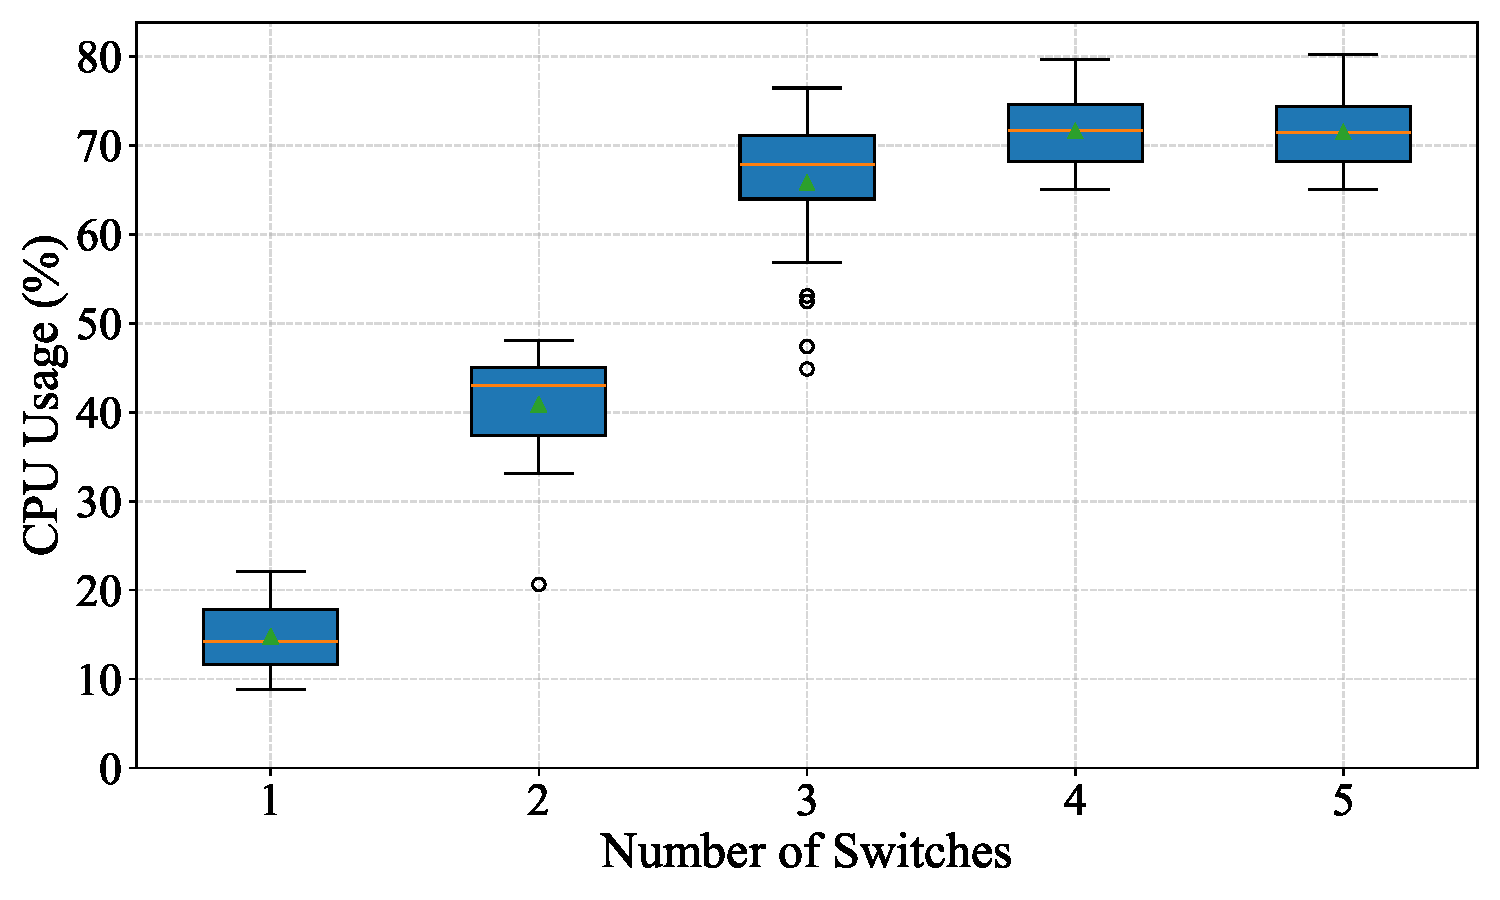
\includegraphics[width=0.49\textwidth]{./figures/cpu_usage_sw.pdf}
    \caption{\rev{Distribution of controller CPU usage under varying numbers of monitored switches.}}
    \label{cpu_usage_sw}
\end{figure}

\subsubsection{\rev{Discussion}}

\rev{
Across both experiments, controller CPU utilization converges to a similar upper bound of approximately 70\%. 
This phenomenon is primarily attributed to the limited computational resources of the experimental environment, where CPU capacity is concurrently consumed by network emulation, traffic generation, machine learning inference, and operating system processes. 
Once the CPU becomes saturated, additional increases in flows or switches do not translate into proportional increases in observed utilization.
}

\rev{
Importantly, this behavior reflects a limitation of the software based testbed rather than an inherent scalability bottleneck of the proposed framework. 
In practical deployments with hardware controllers or dedicated control plane resources, the same adaptive monitoring logic is expected to scale to substantially larger numbers of flows and switches. 
Therefore, the observed saturation indicates stable system behavior under resource constrained conditions, while suggesting that scalability can be further improved with more powerful control plane infrastructure.
}

\rev{
Metrics such as P4Runtime RPC rate, register write latency, and end to end monitoring latency are not separately reported in this evaluation. 
These metrics are tightly coupled with controller CPU load in the adopted software based testbed, and their behavior is largely dominated by overall system resource contention rather than protocol level bottlenecks. 
As a result, controller CPU utilization serves as a representative and conservative indicator of scalability under increasing monitoring scale in the considered environment.
}
